\mychapter{6}{Quality Control}
\label{chap:QC}
The seq-toolbox contains two quality control tools. FastQC \cite{fastqc} and Fast Screen \cite{fast_screen}. Each of these tools serves a different purpose. FastQC offers several sets of analysis which give an indication on the quality of the data, or in other words, if something went wrong with the sequencing process. Fast Screen on the other hand attempts to map reads to a variety of genomes, this can in turn lead to several conclusions about the data. The primary use of Fast Screen is to check if there are contaminations in the data. The standard workflow would be to check the FastQC results, and if these are good, then check the Fast Screen results. Once both of these are found to give good results, the subsequent analysis can be conducted.\\
The `QC\_results' folder in the results folder contains five files. Three for FastQC and two for Fast Screen.\\
\begin{itemize}
\item file ending in fastqc.err: This is an error log that can be consulted if the code crashed. Specifically this error log is for the FastQC pipeline.
\item file ending in fastqc.html: This is the standard FastQC report.
\item file ending in fastqc.zip: This is a compressed folder containing the elements (images and html code) of the FastQC report. This can be relevant if a user wants to extract one or several of the pictures from the report.
\item file ending in screen.html: The html report of Fast Screen
\item file ending in screen.txt: A table/numeric format for the results of Fast Screen
\end{itemize} 

\section{FastQC \label{sec:fastqc}}
In this section we will cover the different elements of the FastQC report. Most of the information covered in this document can be found in more detail on FastQC's main tutorial webpage (\url{https://hbctraining.github.io/Intro-to-rnaseq-hpc-salmon/lessons/qc_fastqc_assessment.html}).\\
Each sub(sub)section below will cover different sections of the FastQC report.

\subsection{Per sequence quality \label{subsec:fastqc_seq_quality}}
\begin{wrapfigure}{r}{0.5\textwidth}
  \begin{center}
    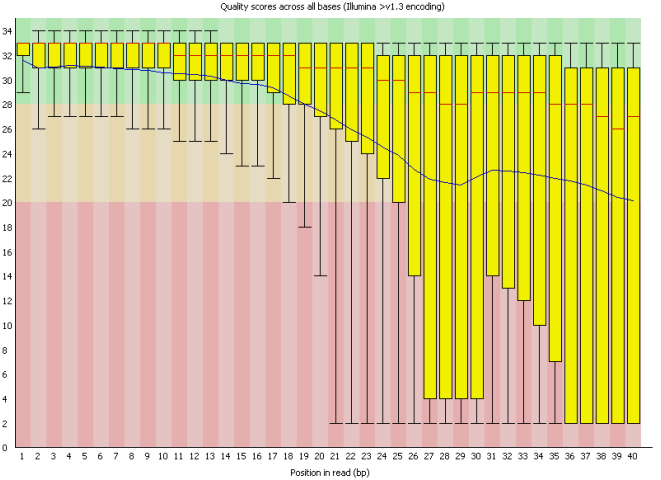
\includegraphics[width=0.5\textwidth]{figures/FastQC_per_base_sequence_quality.png}
  \end{center}
  \label{fig:fastqc_per_seq_qc}
\end{wrapfigure}
\autoref{fig:fastqc_per_seq_qc} shows an example of the per sequence quality graph. This graph essentially provides a quality score per base sequenced. The x axis shows the number of bases, in this case 1 to 40, indicating that at most, 40 bases were sequenced in a row. The y axis represents quality, with the higher score indicating a higher quality. Each instance of the x axis shows a boxplot which represents the quality range (with error margins) of all bases at the number 1 position within the fastq file.\\
If a file is of good quality we expect a majority of early bases to be of high quality (in the green) and the quality would progressively drop as we continue through the x axix, \autoref{fig:fastqc_per_seq_qc} is a good illustration of a good file. However we would hope that the median (red bar in the boxplot) never drops into the lower part of the plot (orange/red color).\\
Things to look out for are abnormal/erratic curves or large `bumps' in the data. Essentially we would expect a relatively smooth curve, if this is not the case we would need to further investigate (using the other elements of this report) to understand if these abnormalities are perhaps an expected biological aspect of the experiment or if something went wrong with the sequencing.\\
The result format seen in \autoref{fig:fastqc_per_seq_qc} also come in a line plot format, in the report this is called `Pre sequence quality scores'.

\subsection{Per base sequence content \label{subsec:fastqc_seq_content}}
\begin{wrapfigure}{r}{0.5\textwidth}
  \begin{center}
    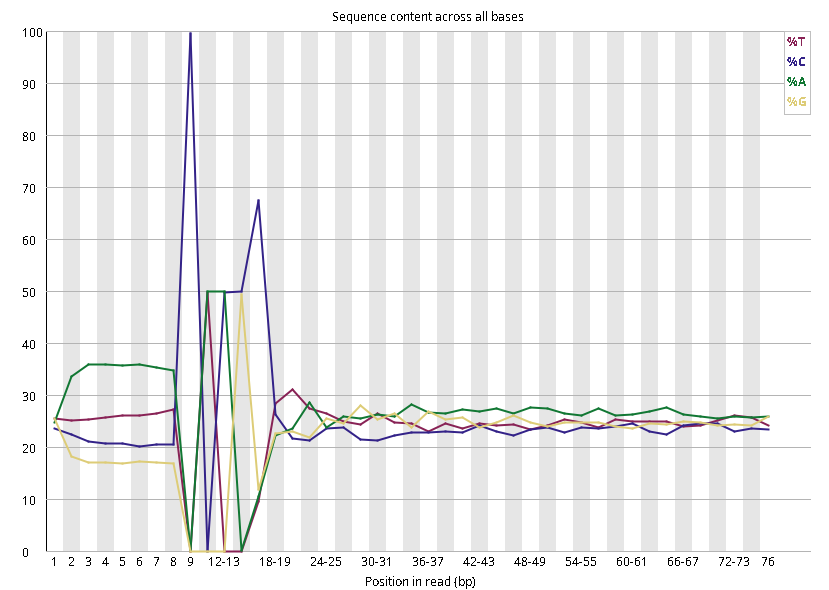
\includegraphics[width=0.5\textwidth]{figures/FastQC_per_base_seq_content.png}
  \end{center}
  \label{fig:fastqc_per_seq_content}
\end{wrapfigure}
As the name indicates this plot shows the distribution of nucleotide type along the x axis of number of bases. Red shows the \%T, blue is \%C, green is \%A, and yellow is \%G. Note that in cases of RNAseq, or other sequencing methods were we include random priming (such as sBLISS) the first n number of bases will likely be erratic, thus throwing an error or warning in the report. For example in \autoref{fig:fastqc_per_seq_content} we see the results of an sBLISS file. The first 8 bases are a bit odd as they represent UMIs, while bases 9-18 are extremely erratic as these are sample barcodes. After this barcode we observe a very normal distribution. Therefore even though FastQC would throw an error for this behaviour, in the context of our experiment it is what we would expect.\\
In the event that strong biases are observed in what would be genomic regions of the file, it is possible that there was a contamination in the library or an error occurred in the sequencing of the library. In either case the error is likely at the lab or sequencing level and not much can be done at the data processing level.

\subsection{Per sequence GC content \label{subsec:fastqc_GC_content}}
\begin{wrapfigure}{r}{0.5\textwidth}
  \begin{center}
    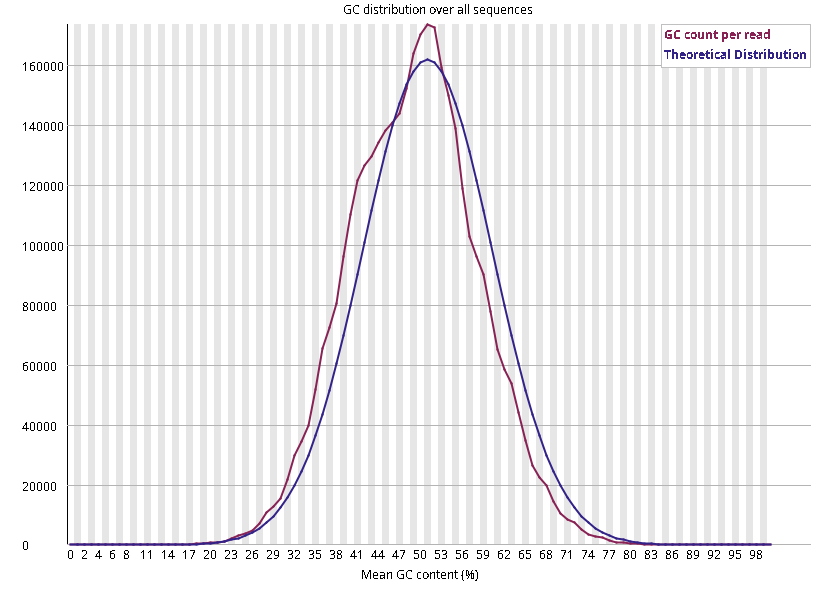
\includegraphics[width=0.5\textwidth]{figures/FastQC_GC_content.png}
  \end{center}
  \label{fig:fastqc_GC_content}
\end{wrapfigure}
For this set of results we expect a normal distribution where the central peak more or less corresponds to the expected GC content for the organism being sequenced. Note that FastQC provides a curve for the theoretical distribution of the GC content (blue curve), however this is calculated based on the data and is not representative of the expected curve for the particular organism. Users can check the work of Romiguier et.al \cite{romiguier2010contrasting} where the expected GC content of 33 different mammals is shown. For convenience, humans are expected at around 46.1\% and mice at 51.24\%. Unfortunately they have not looked at C.elegans, for this we turn towards other studies such as one from John E Sulston and Sydney Brenner \cite{sulston1974dna} which show that the expected GC content for C.elegans is 36\%.\\
In our example dataset taken from an sBLISS protocol we have a human sample whose distribution is slightly shifted \autoref{fig:fastqc_GC_content}. The peak lines up with ~50\% as opposed to 46\%. The cause of this shift may be due to the presence of both UMIs and sample barcodes at the start of each of the sequences, in any case it is not a large shift and would not hinder the continuation of the analysis.\\
If the curve is not a normal distribution or has abnormal bumps it is likely indicative of a contaminated library. This type of issue should be flagged by FastQC. However if the curve is shifted, say in a human sample the peak of the curve lines up with 35\% instead of close to 46\% then FastQC will not flag this as an error although this would be cause for concern. A shift such as this would be reflective of some sort of systemic bias. Another possibility is that the actual curve is far higher than the theoretical curve (same peak location on the x axis but the amplitude on the y-axis is much more significant). In this case it essentially states that the data contains more fragments with GC content than expected. This could be normal or represent a contamination. In the event of a contamination we would expect Fast Screen, a secondary quality control measure, to pick it up.

\subsection{Per base N content \label{subsec:fastqc_N_content}}
In sequencing an `N' is added when the sequencer was incapable of reading a A, T, C, or G. The plots for this section show the percentage of N inclusion at each base position. In an ideal world we see little to no Ns in our data, though it isn't abnormal to see some small bumps here and there, particularly in the higher base numbers (further on the x axis). Though it is subjective, while there are no bumps above the 10\% mark I would consider the data to be okay.

\subsection{Sequence length distribution \label{subsec:fastqc_seq_length}}
\begin{wrapfigure}{r}{0.5\textwidth}
  \begin{center}
    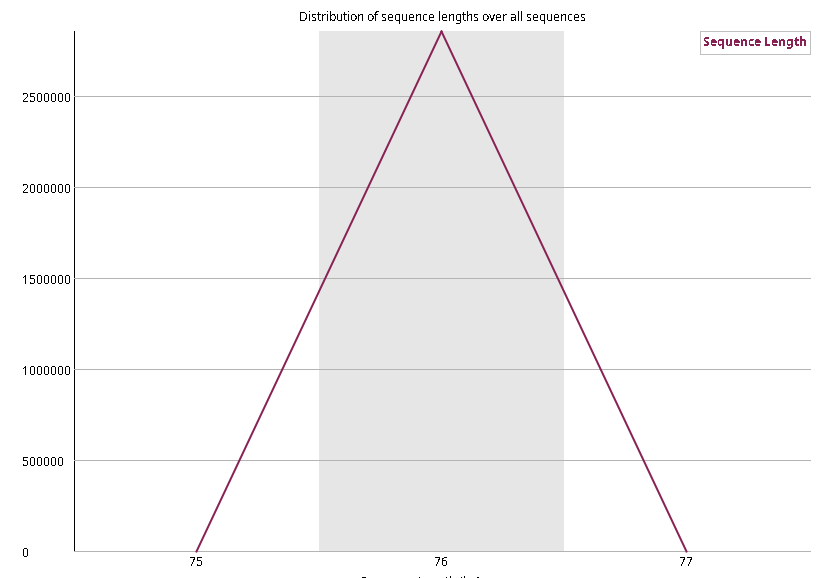
\includegraphics[width=0.5\textwidth]{figures/FastQC_seq_length_distribution.png}
  \end{center}
  \label{fig:fastqc_seq_length}
\end{wrapfigure}
This is another section which is relatively complicated and produces varying results depending on the experiment being done. In addition it isn't the most intuitive set of results. In short, sequencers may generate fragments of uniform lengths or not. The graph of this section shows the distribution of fragment sizes. Generally we expect one large peak, the x axis location of this peak is not incredibly relevant. In our sBLISS examplke dataset seen in \autoref{fig:fastqc_seq_length} we see one large peak at 76bp. This essentially shows that all our reads are 76bp in length. This is a concrete example of a uniform size distribution. This link(\url{https://www.bioinformatics.babraham.ac.uk/projects/fastqc/Help/3\%20Analysis\%20Modules/7\%20Sequence\%20Length\%20Distribution.html}) shows an example of a non-uniform distribution of sizes. The cases where this plot would show cause for concern is if the curve of a non-uniform distribution is erratic, or if the length is much shorter than expected.

\subsection{Sequence Duplication Levels \label{subsec:fastqc_seq_dup}}
\begin{wrapfigure}{r}{0.5\textwidth}
  \begin{center}
    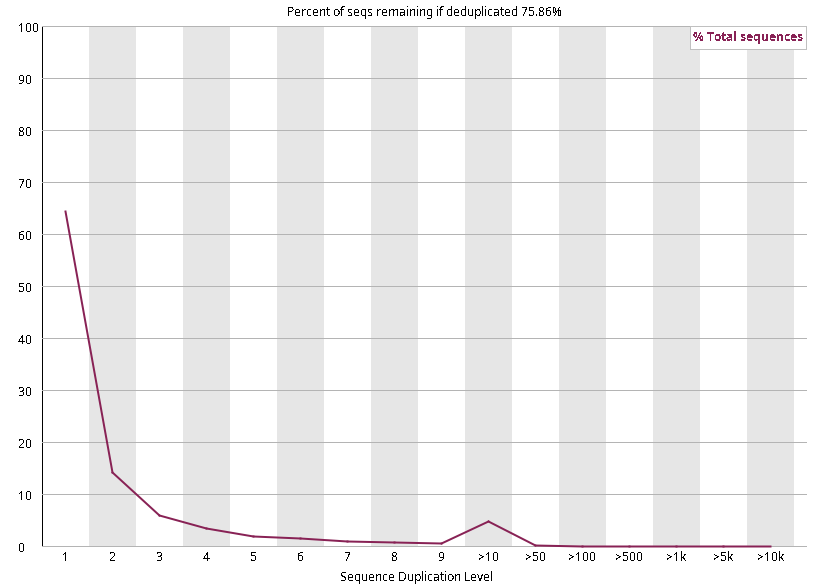
\includegraphics[width=0.5\textwidth]{figures/FastQC_seq_dups.png}
  \end{center}
  \label{fig:fastqc_seq_dups}
\end{wrapfigure}
As the name implies this plot shows the level of duplicated sequences. The y axis is a percentage while the x axis is a duplication level. The plot, fragments (or sequences) which are only observed once are found on the `1' of the x axis. Sequences which are found twice are on the `2' of the x axis and so on. The y axis therefore shows us the percentage of sequences which appear once, twice, and so on until we've checked all sequences.\\
In an ideal world we would expect a large peak at `1' on the x axis and a sharp drop off to then have a plateau at 0. Depending on the type of experiment performed this may not always occur. For example in our sBLISS results \autoref{fig:fastqc_seq_dups} we see the `ideal' scenario however there is a small bump at the 10th level. This indicates that there is a small group of fragments which are very overrepresented. Within the context of our data we assume that this is due to the presence of the sample barcode (adaptors). If these were to be trimmed (removed) this bump would likely disappear.\\
Another possibility is to observe a sharp peak on the later end of the plot, this would indicate that the library used is not very diverse and therefore most fragments have been sequenced multiple times over. This is not inherently an error, but it does show that money may be saved by diversifying, or mixing the library in future iterations of the sequencing.\\
In other instances bump in the curve may appear throughout the plot showing that there are varying levels of duplication. This kind of situation could be either technical or biological in nature. There is no guideline for this kind of event other than attempting to find a biological cause for this behaviour, if one cannot be found it is likely technical in origin. Note that RNAseq often has this kind of profile as in order to observe very scarce fragments, we would inevitably have to over-sequence the prevalent fragments.\\
NOTE: FastQC does not actually check all sequences for this module as this would not be memory efficient from a computing perspective. Instead it creates these results for the first 200 000 sets of sequences. These results are still important, however it is noteworthy to understand that they are not representative of the entire file.

\subsection{Overrepresented sequences \label{subsec:fastqc_overrep}}
This one is a bit more straight-forward. This section will show you if a or several particular sequences/fragments are overrepresented in the file. This could mean that these sequences are of particular importance or it could mean that they are some sort of contamination. All sequences appearing more than 0.1\% of the total are shown. It is likely that if `bumps' are seen in the sequence duplication levels that the cause of these bumps appears in the overrepresented sequences. This may provide the opportunity to identify the cause: contamination, biological significance, or perhaps adapters ect...\\
Note that only the first 200 000 sequences are queried and therefore the results are considered an overview, they do not represent the entirety of the data.


\subsection{Adapter content \label{subsec:fasctqc_Adapter}}
This area simply shows the presence of certain adapter types along the found sequences. This plot can be a helpful tool to customize the trimming component of the pipeline \autoref{sec:trimming}. However in most cases a customized trimming will not be required.

\section{Fast Screen \label{sec:Fast_Screen}}
Fast screen is a much simpler quality control tool when compared to FastQC. In short, Fast Screen attempts to map the found sequences to several genomes. This is meant to serve as a means to evaluate contamination presence and amounts.\\
The results are shown as an HTML file and TXT file, with the HTML file containing a table and plot while the TXT file only contains the table.\\
As an example, \autoref{tab:fast_screen} shows the Fast Screen results for one of the example control files in an sBLISS experiment. Specifically this file contained human data. The important columns are the hits/multi-hits column as these indicate where reads have been mapped. In an ideal world all reads are one hit to one genome, with that genome being the one you sequenced. Having multiple hits on a single genome is to be expected as well. Some possible cases are discussed below.\\
\clearpage
\begin{itemize}
\item Good sample - illustrated in \autoref{tab:fast_screen}.\\
There are mostly hits on a single genome, with some hits on adapters. In this case hits on adapters are expected due to the nature of the sBLISS protocole (see \autoref{sec:sBliss_adaptors}).
\item Contaminated samples\\
In the case of contaminated samples we would likely see several `one genome' results across multiple genomes. This would be a clear sign of contamination.
\item Low complexity reads\\
In this scenario we expect to see mostly multiple-genome results and very few single genome results. This means that the reads obtained are of insufficient quality to be reliably mapped.
\end{itemize}
\begin{table}
\small
\caption{Table showing the results of Fast Screen on one of the example control samples for the sBLISS pipeline} 
\begin{tabular}{|p{.11\textwidth}|p{.05\textwidth}|p{.1\textwidth}|p{.12\textwidth}|p{.12\textwidth}|p{.15\textwidth}|p{.15\textwidth}|}
 \hline
 Genome & Reads & Unmapped & \makecell{One hit/\\one genome} & \makecell{Multi-hits/\\one genome} & \makecell{One hit/\\multi-genomes} & \makecell{Multi-hits/\\multi-genomes}\\
 \hline
 Human & 98403 & 19666 & 53470 & 18418 & 653 & 6196\\
 \hline
 Mouse & 98403 & 93107 & 8 & 5 & 1419 & 3864\\
 \hline
 Rat & 98403 & 92647 & 11 & 6 & 948 & 4791\\
 \hline
 Drosophila & 98403 & 97183 & 1 & 1 & 227 & 991\\
 \hline
 Worm & 98403 & 97872 & 5 & 0 & 274 & 252\\
 \hline
 Yeast & 98403 & 97782 & 0 & 0 & 22 & 599\\
 \hline
 Arabidopsis & 98403 & 97482 & 0 & 0 & 225 & 696\\
 \hline
 Ecoli & 98403 & 98403 & 0 & 0 & 0 & 0\\
 \hline
 rRNA & 98403 & 95075 & 0 & 13 & 79 & 3236\\
 \hline
 MT & 98403 & 98153 & 0 & 0 & 234 & 16\\
 \hline
 PhiX & 98403 & 98403 & 0 & 0 & 0 & 0\\
 \hline
 Lambda & 98403 & 98403 & 0 & 0 & 0 & 0\\
 \hline
 Vectors & 98403 & 98036 & 7 & 0 & 272 & 88\\
 \hline
 Adapters & 98403 & 92235 & 1403 & 4502 & 0 & 263\\
 \hline
\end{tabular}
\label{tab:fast_screen}
\end{table}

\section{MAPQ\label{sec:MAPQ}}
MAPQ stands for MAPping Quality. Unfortunately MAPQ suffers from having multiple methods and definitions depending on the tool used. Samtools sets MAPQ as a range of 0 to 255 with 255 being high confidence mapping. MAPQ is calculated by mappers and some seem to have set ceilings, although this is not explicit in their documentation. Some blog posts have found that bwa has a maximum threshold of 37 while bowtie2 has a maximum of 42 (\url{https://www.acgt.me/blog/2014/12/16/understanding-mapq-scores-in-sam-files-does-37-42}). However bwa has two methods of mapping, one which results in a maximum score of 37 while the other gives a maximum score of 60. This means that for bwa mapped files which used `mem', a q threshold of 60 is essentially selecting for the best confidence possible.\\
This not only illustrates the difficulty in using the MAPQ metric, but also it's inconsistency. This constitutes a relatively large point of debate in the bioinformatic community, that is if MAPQ scores can be trusted/used. There is no widely accepted consensus.\\
This toolbox will use what the pipelines contained within it originally come with, for example sBLISS filters for a MAPQ of 60 when using BWA, meaning the highest confidence of mapping from this tool. GLOE-seq uses a filter of 30 for a bowtie2 aligned file, with bowtie2 having a maximum cap of 42. Based on the way bowtie2 does it's calculation this filter mostly removes reads that are considered to be multi-mapped, that is they can be mapped to more than one location on the genome.\\
In the event where the toolbox is not following a set pipeline no MAPQ filter will be applied. \todo{update with final opinion.}

\section{QualiMap \label{sec:qualimap}}
Qualimap is a tool to perform some quality control metrics on aligned data \cite{qualimap,qualimap2}. This tool differs from previously discussed tools such as Fastqc (\autoref{sec:fastqc}) which perform quality control on as of yet unaligned data. Though the uses of qualimap are diverse this toolbox uses the basic function called bamqc which generates a pdf report on the quality of a single BAM file. There is some overlap between Fastqc and bamqc, with the main similarity being that they both give measure of GC content distribution as well as mapped reads nucleotide content (per base sequence content), for these elements, refer to \autoref{subsec:fastqc_GC_content} and \autoref{subsec:fastqc_seq_content} respectively. Bamqc also covers duplicated reads, similar to \autoref{fig:fastqc_seq_dups}. Below we cover the elements that are unique to bamqc.\\

\subsection{Coverage across reference \label{subsec:bamqc_coverage}}
\begin{wrapfigure}{r}{0.5\textwidth}
  \begin{center}
    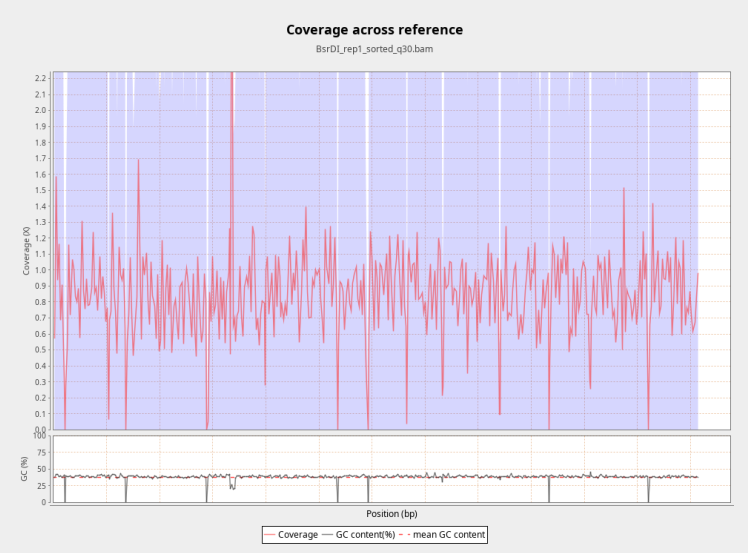
\includegraphics[width=0.5\textwidth]{figures/bamqc_coverage.png}
  \end{center}
  \label{fig:bamqc_coverage}
\end{wrapfigure}
The upper figure shows the coverage distribution while the lower shows the GC content across the reference (black line). The coverage metric (X) equates to the number of reads mapped to each nucleotide of the region, an example can be seen in \autoref{fig:bamqc_coverage}. Put simply, the larger the coverage the more reads in that location of the reference genome. In practice one would expect this graph to relatively inconsistent across the x axis, in other words the coverage is expected to fluctuate quite a bit. In cases where reads are very specific to a location of the genome, one could expect to see a sharp peak at one or few locations as opposed to constant fluctuation. To best utilize this graph one should assess what the protocol has measured and if the expected results correlate with the behaviour seen in this graph. These results are also shown as a histogram which shows the number of reads (y axis) mapped to which coverage (x axis). This histogram also comes with a 50X coverage variant in the event that certain areas of the genome are highly targetted.\\
Similarly there is a plot covering the `Genome Fraction Coverage' which shows the fraction/percentage of the reference associated to a coverage value. It serves as yet another form of visualization for the coverage across the reference.

\subsection{Homopolymer Indels \label{subsec:bamqc_homopolymer}}
\begin{wrapfigure}{r}{0.5\textwidth}
  \begin{center}
    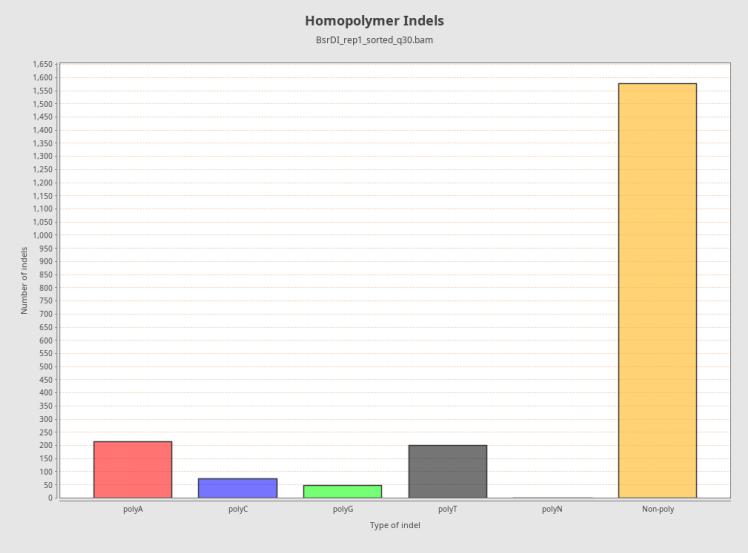
\includegraphics[width=0.5\textwidth]{figures/bamqc_homopolymer.png}
  \end{center}
  \label{fig:bamqc_homopolymer}
\end{wrapfigure}
If indels are present in the dataset, this plot (\autoref{fig:bamqc_homopolymer}) is generated. The official definition of this plot is "this plot shows separately the number of indels that are within a homopolymer of A’s, C’s, G’s or T’s together with the number of indels that are not within a homopolymer". In the context of DNA, a homopolymer is a series of identical nucleotides, perhaps the most common example being a polyA tail. BamQC defines a homopolymer as being at least 5 consecutive identical nucleotides. Homopolymers are known to cause difficulties in sequencing in addition to having increased error rates when compared to other areas of the genome \cite{kunkel2004dna,fazekas2010improving}. This metric on it's own cannot say if a mapping is good or bad, but it can serve as an indication of the certainty of mapping for areas which are rich in homopolymers. This can be taken into account when interpreting results. In the event that the amount of indels are overwhelmingly high it may indicate an issue with the sequencing itself. In the example figure given the statistic if roughly 25\% of reads are indels (this value is found in a table of the report but not in the plot). This would be a case where the amounts would be considered `overwhelmingly high'. In this case, the dataset originates from an example fastq file which is not expected to produce meaningful results.

\subsection{Mapping Quality Histogram \label{subsec:bamqc_mapq}}
\begin{wrapfigure}{r}{0.5\textwidth}
  \begin{center}
    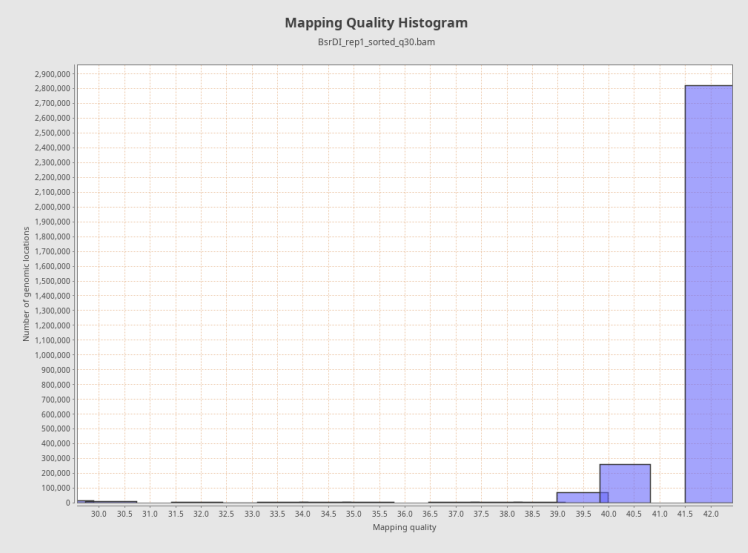
\includegraphics[width=0.5\textwidth]{figures/bamqc_mapq.png}
  \end{center}
  \label{fig:bamqc_mapq}
\end{wrapfigure}
This plot gives a visual representation of the quality of mapping (MAPQ). More information about this metric can be found in \autoref{sec:MAPQ}. This graph is quite useful in determining if the file could benefit from a MAPQ based filter. In the case of \autoref{fig:bamqc_mapq} the results shows scores only above the 30 score as this BAMQC was performed on a bam file which has already been submitted to a MAPQ filter of 30.